\documentclass[12pt, a4paper]{article}

% Ru lang stuff
\usepackage [utf8x] {inputenc}
\usepackage [T2A] {fontenc}

% running titles 
\usepackage{fancybox}
\usepackage{fancyhdr}

% for last page number
\usepackage{lastpage}

%for colored tablets cells
\usepackage{colortbl}

% for Ru text in formulas
\usepackage[warn]{mathtext}

% for captions 
\usepackage[labelsep=period]{caption}
\usepackage{capt-of}

% for colored hyperrefs
\usepackage{xcolor}
\usepackage{hyperref}

% for pictures 
\usepackage{graphicx}

% for coll math
\usepackage{amsmath}

% path to all pictures
\graphicspath{{picks/}}

% for enumerates
\usepackage[shortlabels]{enumitem}

% for diff running titles on pages with diff parity
\usepackage{ifthen}
\usepackage{pdfpages}
\usepackage[strict]{changepage}

% for graphics
\usepackage{pgfplots}
\pgfplotsset{compat=1.9}

%for drawings
\usepackage{tikz}
\usetikzlibrary{calc}
\usetikzlibrary{decorations.pathmorphing}

% for good text in tablets
\usepackage{array}

% upgrading tables
\newcolumntype{P}[1]{>{\centering\arraybackslash}p{#1}}
\newcolumntype{M}[1]{>{\centering\arraybackslash}m{#1}}


% dock fields 20 15 15 35
\usepackage[left=12mm, top=12mm, right=15mm, bottom=28mm, nohead, footskip=10mm]{geometry}

% for cool tables
\usepackage{multirow}

% for different section/subsection/subsubsection styles in contents and doc
\usepackage[english, russian]{babel}

\usepackage{amsmath}

% for cool tables
\usepackage{tabularx}

\newcommand{\sect}[2] {
    \addtocounter{section}{1}
    \section*{\Huge\thesection.\,#1}
    \addcontentsline{toc}{subsection}{ \texorpdfstring{\thesection.\qquad\qquad #2}{Lg}}
}

\newcommand{\subsec}[2] {
    \addtocounter{subsection}{1}
    \subsection*{\thesubsection.\,#1}
    \addcontentsline{toc}{subsection}{ \texorpdfstring{\quad \thesubsection.\qquad\ #2}{Lg}}
}

\newcommand{\subsubsec}[2] {
    \addtocounter{subsubsection}{1}
    \subsubsection*{\thesubsubsection.\,#1}
    \addcontentsline{toc}{subsection}{ \texorpdfstring{\quad\quad\ \thesubsubsection. #2}{Lg}}
}
%-------------------------------------------------------------------------%

% for easy mini pages with shifts
\newcommand{\shiftedText}[3]{
\hspace*{#1}\begin{minipage}[t]{#2}
#3
\end{minipage}
}

\newcolumntype{P}[1]{>{\centering\arraybackslash}p{#1}}

% page style setup (for running titles)
\fancypagestyle{plain}{ %
\fancyhf{} % remove everything

 % lines parameters
\renewcommand{\headrulewidth}{0pt}
\renewcommand{\footrulewidth}{0pt}

% running titles contents
\fancyfoot[L]{\ifthenelse{\isodd{\thepage}}{Работа 1.2.5}{\thepage}}
\fancyfoot[R]{\ifthenelse{\isodd{\thepage}}{\thepage}{Работа 1.2.5}}
}

% choosing page style with our running titles
\pagestyle{plain}

\tolerance = 10000

\title{Лабораторная работа №1.2.5}
\author{Mikhail Pavlov \thanks{MIPT}}
\date{December, 2021}
\begin{document}


\shiftedText{0.5cm}{14cm}
{
    \begin{center}
    \vspace*{1.0cm}    
        
        {\bf\Huge Работа 1.2.5 }
        
    \vspace*{0.2cm}    
        
        {\bf\LARGE Исследование прецессии уравновешенного гироскопа. }
        
    \vspace*{0.8cm}
        {\LARGE Работу выполнил Павлов Михаил Б01-109 }
        
    \vspace*{1.6cm}
    
    \end{center}
}

\fancypagestyle{plain}{ %
\fancyhf{} % remove everything

 % lines parameters
\renewcommand{\headrulewidth}{0pt}
\renewcommand{\footrulewidth}{0pt}
% running titles contents
\fancyfoot[L]{\ifthenelse{\isodd{\thepage}}{Работа 1.2.5}{\thepage}}
\fancyfoot[R]{\ifthenelse{\isodd{\thepage}}{\thepage}{Работа 1.2.5}}
}

% choosing page style with our running titles
\pagestyle{plain}

\tolerance = 10000

\vspace*{0.6cm}

\section{Аннотация}

В работе исследуется вынужденная прецессия гироскопа. Устанавливается зависимость скорости вынужденной прецессии от величины момента сил,
действующих на ось гироскопа. Определяется скорость вращения ротора гироскопа и сравнивается со скоростью, рассчитанной по скорости прецессии. 

\section{Теоретический сведения}

Уравнение движения твёрдого тела можно записать в следующем виде:

\begin{equation}
\frac{d\vec{P}}{dt}=\vec{F}
\label{one}
\end{equation}

\begin{equation}
\frac{d\vec{L}}{dt}=\vec{M}
\label{two}
\end{equation}

Момент импульса тела в главных его осях $x$, $y$, $z$ равен

\begin{equation}
\vec{L} = \vec{i}I_x\omega_x+\vec{j}I_y\omega_y+\vec{k}I_z\omega_z,
\label{three}
\end{equation}
где $ I_x $, $ I_y $, $ I_z $ -- главные моменты инерции, $ \omega_x $, $ \omega_y $, $ \omega_z $ -- компоненты вектора угловой скорости $ \vec{\omega} $. Быстро вращающееся тело, для которого, например,

\begin{equation}
I_z\omega_z \gg I_x\omega_x,\;\;\;\;I_y\omega_y,
\end{equation} 
принято называть гироскопом. Гироскоп называется уравновешенным, если его центр масс неподвижен.

В силу {two} приращение момента импульса определяется интегралом

\begin{equation}
\Delta\vec{L} = \int\vec{M} dt.
\label{four}
\end{equation}
Если момент внешних сил действует в течение короткого промежутка времени, из интеграла {four} следует, что приращение $ \Delta \vec{L} $ момента импульса значительно меньше самого момента импульса:

\begin{equation}
\left|\Delta \vec{L}\right| \ll \left|\vec{L}\right| 
\end{equation}

\noindent\begin{minipage}[c]{0.4\textwidth}
    \hspace{1cm}
    С этим связана замечательная устойчивость, которую приобретает движение гироскопа после приведения его в быстрое вращение. 
Выясним, какие силы надо приложить к гироскопу, чтобы изменить 
направление его оси. Рассмотрим для 
примера маховик, вращающийся вокруг оси $ z $, перпендикулярной к плоскости маховика (рис. 1). Будем считать, что

\begin{equation}
    \omega_z = \omega_0, \;\;\;\;\; \omega_x = 0, \;\;\;\;\; \omega_y = 0.
    \end{equation}
    
    \noindent Пусть ось вращения повернулась в плоскости $ zx $ по направлению к оси $ x $ на бесконечно малый угол $ d\varphi $. Такой поворот означает добавочное вращение маховика вокруг оси $ y $, так что

    \begin{equation}
    d\varphi=\Omega dt,
    \end{equation}

\end{minipage}
\begin{minipage}[c]{0.57\textwidth}
    \begin{center}
        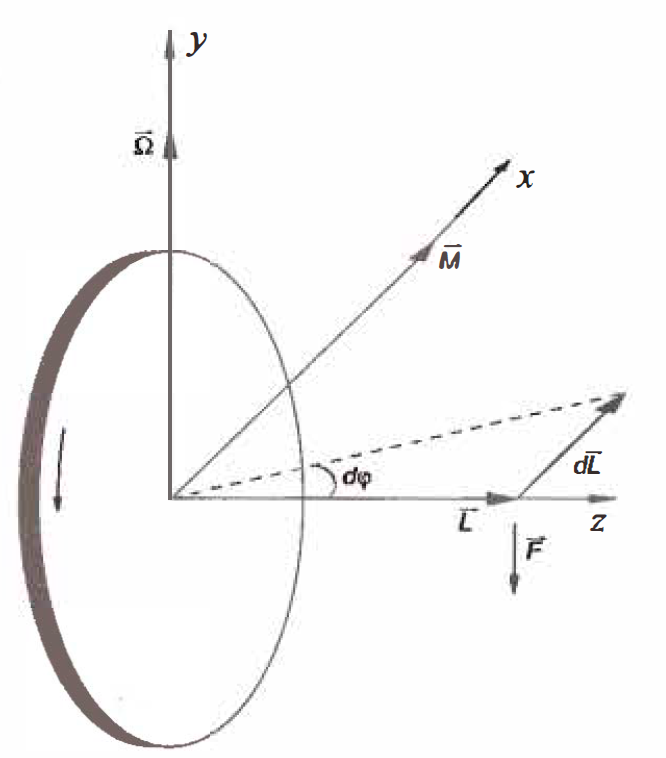
\includegraphics[scale=0.58]{Pics/picture1.png} \\
        \textit{\textcolor[HTML]{000000}{Рис. 1. Маховик}}
    \end{center}
\end{minipage}  

где $ \Omega $ -- угловая скорость такого вращения. Будем предполагать, что

\begin{equation}
L_\Omega \ll L_{\omega_0}
\label{five}
\end{equation}
Это означает, что момент импульса маховика, равный $ I_z\omega_0 $ до приложения внешних сил, только повернётся в плоскости $ zx $ по направлению к оси $ x $, не изменяя своей величины. Таким образом, 

\begin{equation}
\left|d\vec{L}\right| = Ld\varphi = L\Omega dt.
\end{equation}
Но это изменение направлено вдоль оси $ x $, поэтому вектор $ d\vec{L} $ можно представить в виде векторного произведения вектора угловой скорости $ \omega $, направленного вдоль оси $ y $, на вектор собственного момента импульса маховика, направленного вдоль оси $ z $,

\begin{equation}
d\vec{L}=\vec{\Omega} \times \vec{L} dt,
\end{equation}
т. е.

\begin{equation}
\frac{d\vec{L}}{dt} = \vec{\Omega} \times \vec{L}.
\end{equation}
В силу {two} имеем

\begin{equation}
\vec{M} = \vec{\Omega} \times \vec{L}.
\label{six}
\end{equation}
Формула {six} справедлива, если выполнено условие {five}. Она позволяет определить момент сил $ \vec{M} $, который необходимо приложить к маховику для того, чтобы вызвать вращение оси маховика с угловой скоростью $ \vec{\Omega} $. Мы видим, таким образом, что для поворота оси вращающегося маховика к оси $ x $ необходимо приложить силы, направленные не вдоль оси $ x $, а вдоль оси $ y $, так чтобы их момент $ \vec{M} $ был направлен вдоль оси $ x $.

Для гироскопа массой $ m_\text{г} $, у которого ось собственного вращения наклонена на угол $ \alpha $ от вертикали, скорость прецессии, происходящей вокруг вертикальной оси под действием силы тяжести, равна

\begin{equation}
\Omega = \frac{M}{I_z\omega_0\sin \alpha} = \frac{m_\text{г}gl_\text{ц}\sin\alpha}{I_z\omega_0\sin\alpha} = \frac{m_\text{г}gl_\text{ц}}{I_z\omega_0},
\end{equation}
где $ l_\text{ц} $ -- растояние от точки подвеса до центра масс гироскопа, т. е. скорость прецессии не зависит от угла $ \alpha $.

Для изучения регулярной прецессии уравновешенного гироскопа к его оси подвешивают дополнительные грузы. Это смещает общий центр масс и создает момент сил тяжести, вызывающий прецессию. Скорость прецессии в этом случае равна

\begin{equation}
\Omega = \frac{mgl}{I_z\omega_0},
\label{eight}
\end{equation}
где $ m $ -- масса груза, $ l $ -- расстояние от центра карданова подвеса до точки крепления груза на оси гироскопа.

Измерение скорости прецессии гироскопа позволяет вычислить угловую скорость вращения его ротора. Расчет производится по формуле {eight}. Момент инерции ротора относительно оси симметрии $ I_0 $ измеряется по крутильным колебаниям точной копии ротора, подвешиваемой вдоль оси симметрии на жесткой проволоке. Период крутильных колебаний $ T_0 $ зависит от момента инерции $ I_0 $ и модуля кручения проволоки $ f $:

\begin{equation}
T_0 = 2\pi\sqrt{\frac{I_0}{f}}.
\label{nine}
\end{equation} 

Чтобы исключить модуль кручения проволоки, вместо ротора гироскопа к той же проволоке подвешивают цилиндр правильной формы с известными размерами и массой, для которого легко можно вычислить момент инерции $ I_\text{ц} $. Для определения момента инерции ротора гироскопа имеем 

\begin{equation}
I_0=I_\text{ц}\frac{T_0^2}{T_\text{ц}^2},
\label{ten}
\end{equation}
где $ T_\text{ц} $ --период крутильных колебаний цилиндра.


\section{Экспериментальная установка}

Экспериментальная установка для исследования прецессии уравновешенного гироскопа показана на рис. 2.
Ротором гироскопа является ротор высокооборотного электромотора М, питающегося током частотой 400 Гц.
Кожух мотора (статор, имеющий обмотки, питаемые током частотой 400 Гц) скреплен с кольцом Б.
Мотор с кольцом Б может вращаться в кольце А вокруг горизонтальной оси, которое может вращаться вокруг вертикальной оси.
Ротор электромотора представляет массивный стальной цилиндр с прожилками меди, образующими "беличье колесо".
Обозначенный на рисунке буквой С рычаг направлен по оси симметрии ротора. На рычаг подвешивают грузы Г.
Подвешивая различные грузы, можно менять силу $F$, момент которой определяется расстоянием $l$ от точки подвеса до горизонтальной оси кольца А
(до центра масс гироскопа), указанным на самой установке.

\begin{center}
    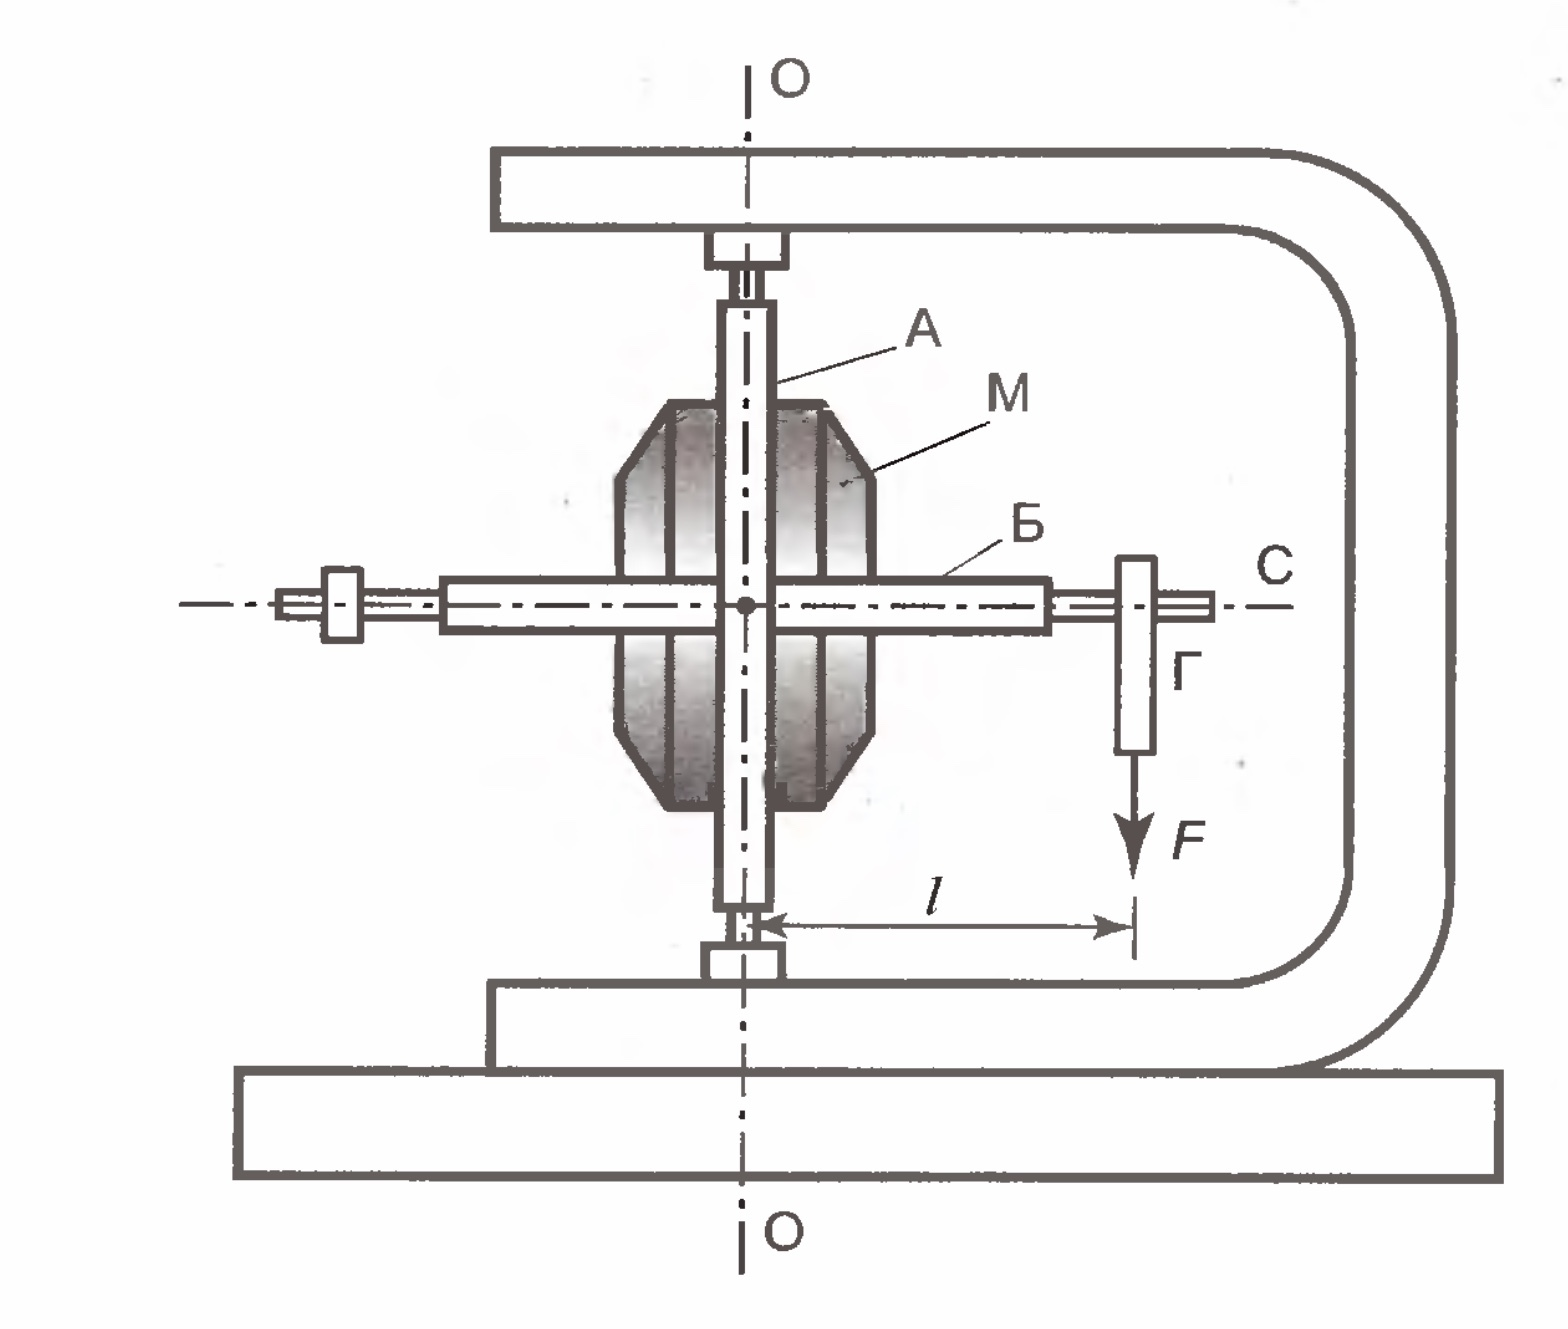
\includegraphics[scale=0.3]{Pics/picture2.jpg} \\
    \textit{\textcolor[HTML]{000000}{Рис. 2. Схема установки}}
\end{center}

{\large Инструментальные погрешности \\}
\textbf{Линейка: } $\sigma_{rul} = \pm 1$ мм (цена деления)\\
\textbf{Электронные весы: } $\sigma_{v} = \pm 10^{-3}$ г (маркировка производителя) \\
\textbf{Штангенциркуль: } $\sigma_{cal} = \pm 0.1$ мм (маркировка производителя) \\
\textbf{Секундомер: } $\sigma_{f} = \pm 0.5$ с (с учетом реакции человека) \\

\section{Результаты измерений и обработка результатов}

{\large Вычисление момента инерции цилиндра \\}

Момент инерции цилиндра можно вычислить по следующей формуле:

\begin{equation}
I_\text{ц} = \frac{1}{2}m_\text{ц}\left( \frac{d_\text{ц}}{2}\right)^2,
\end{equation}
где $ m_\text{ц} $ -- масса цилиндра, $ d_\text{ц} $ -- его диаметр.

При измерении этих параметров получаем:
\begin{itemize}
	\item $ m_\text{ц} = \left( 1617.2 \pm 0.1\right) $ г
	\item $ d_\text{ц} = \left( 76.1 \pm 0,1 \right) $ мм
\end{itemize}

Тогда

\begin{equation}
I_\text{ц} = 1.17 \cdot 10^{-3} \text{ кг} \cdot \text{м}^2
\end{equation}

Погрешность вычисления момента инерции цилиндра может быть найдена по следующей формуле:

\begin{equation}
\sigma_{I_\text{ц}} = I_\text{ц}\sqrt{\left( \frac{\Delta_\text{вес}}{m_\text{ц}} \right)^2 + \left(2 \frac{\Delta_\text{лин}}{d_\text{ц}} \right)^2 } \approx 0.03 \cdot 10^{-3} \text{ кг} \cdot \text{м}^2
\end{equation}

В итоге получаем:

\begin{itemize}
	\item \underline{$ I_\text{ц} = \left(1.17 \pm 0.03 \right) \cdot 10^{-3} \text{ кг} \cdot \text{м}^2 $, $ \left( \varepsilon = 2,6 \% \right) $}
\end{itemize}

{\large Измерение периода крутильных колебаний пробного цилиндра }

Производим измерение времени 15 крутильных колебаний цилиндра и повторяем опыт $ N_\text{оп} = 6 $ раз. Полученные результаты заносим в таблицу 1.

\begin{table}[h!]
	\centering
	\begin{tabular}{|c|c|c|c|c|c|c|}
		\hline
		№ & $ t $, с & $ N_\text{кол} $ & $ T $, с & $ \langle T \rangle $, с                & $ \sigma_T $, с             & $ \varepsilon_T, \% $                      \\ \hline
		1 & 59.9 & 15              & 3.993     & \multirow{6}{*}{3.998} & \multirow{6}{*}{0,016} & \multirow{6}{*}{0,4}      \\ \cline{1-4}
		2 & 59.6 & 15              & 3.973     &                        &                        &                            \\ \cline{1-4}
		3 & 60.1 & 15              & 4.007     &                        &                        &                            \\ \cline{1-4}
        4 & 59.9 & 15              & 3.993     &                        &                        &                            \\ \cline{1-4}
        5 & 60.0 & 15              & 4.000     &                        &                        &                            \\ \cline{1-4}
        6 & 60.3 & 15              & 4.020     &                        &                        &                            \\ \hline
	\end{tabular}
	\caption{Результат измерения периода крутильных колебаний цилиндра}
\end{table}

Период колебаний цилиндра в отдельном опыте может быть рассчитан по формуле:

\begin{equation}
T = \frac{t}{N_\text{кол}}.
\end{equation}

Среднее значение периода крутильных колебаний можно найти по формуле:

\begin{equation}
\langle T \rangle = \frac{1}{N_\text{оп}}\sum_{i = 1}^{N_\text{оп}} T_i.
\end{equation}

Случайную погрешность определения периода крутильных колебаний рассчитываем по формуле:

\begin{equation}
\sigma^{\text{сл}}_T = \sqrt{\frac{1}{N_\text{оп} - 1} \sum_{i = 1}^{N_\text{оп}} \left(T_i - \langle T \rangle \right)^2}.
\end{equation}

Полная погрешность может быть вычислена по формуле:

\begin{equation}
\sigma_T = \sqrt{\left( \sigma^\text{сл}_T \right)^2 + \left( \sigma\text{сек} \right)^2  }
\end{equation}

В итоге получаем:

\begin{itemize}
	\item \underline{$ T_\text{ц} = \left( 3.998 \pm 0,016\right) $ с, $ \left(\varepsilon = 0,4 \% \right)  $}
\end{itemize}

{\large Измерение периода крутильных колебаний ротора гироскопа}

Производим измерение времени крутильных колебаний цилиндра и повторяем опыт 6 раз. Полученные результаты заносим в таблицу.

\begin{table}[h!]
	\centering
	\begin{tabular}{|c|c|c|c|c|c|c|}
		\hline
		№ & $ t $, с & $ N_\text{кол} $ & $ T $, с & $ \langle T \rangle $, с                & $ \sigma_T $, с             & $ \varepsilon_T , \%$                 \\ \hline
		1 & 63.69 & 20              & 3.185     & \multirow{6}{*}{3,184} & \multirow{6}{*}{0,011} & \multirow{6}{*}{0.35} \\ \cline{1-4}
		2 & 63.75 & 20              & 3.188     &                        &                        &                       \\ \cline{1-4}
        3 & 63.50 & 20              & 3.175     &                        &                        &                       \\ \cline{1-4}
        4 & 63.72 & 20              & 3.186     &                        &                        &                       \\ \cline{1-4}
        5 & 63.72 & 20              & 3.186     &                        &                        &                       \\ \cline{1-4}
		6 & 63.62 & 20              & 3.181     &                        &                        &                       \\ \hline
	\end{tabular}
	\caption{Результат измерения периода крутильных колебаний ротора гироскопа}
\end{table}

В итоге получаем:

\begin{itemize}
	\item \underline{$ T_0 = \left( 3.184 \pm 0,011 \right) $ с, $ \left( \varepsilon = 0.35 \% \right)  $}
\end{itemize}


{\large Вычисление момента инерции ротора гироскопа}

Вычислим момент инерции ротора гироскопа:

\begin{equation}
I_0=I_\text{ц}\frac{T_0^2}{T_\text{ц}^2} = 7.80 \cdot 10^{-4} \text{ кг} \cdot \text{м}^2.
\end{equation}
Погрешность вычисления момента инерции ротора гироскопа можно вычислить по формуле:

\begin{equation}
\sigma_{I_0} = I_0\sqrt{\left( \varepsilon_{I_\text{ц}} \right)^2 +\left( 2 \varepsilon_{T_0} \right)^2 + \left(2 \varepsilon_{T_\text{ц}} \right)^2} \approx 0.08 \cdot 10^{-4} \text{ кг} \cdot \text{м}^2.
\end{equation}

В итоге получаем: \label{inertion}

\begin{itemize}
	\item \underline{$ I_0 = \left( 7.8 \pm 0.08 \right) \cdot 10^{-4} \text{ кг} \cdot \text{м}^2, \left( \varepsilon = 1.02   \% \right) $}
\end{itemize}

{\large Определение частоты вращения ротора гироскопа}

\begin{table}[h!]
	\centering
	\begin{tabular}{|c|c|c|c|c|c|c|c|c|c|c|c|c|c|c|c|c|c|}
		\hline
		№  & $ m $, кг          & $ l $, м            & $ M $, Н$\cdot$м      & $ \sigma_M $, Н$\cdot$м             & $ t $, с & $ N_\text{об} $ & $ T $, с & $ \langle T \rangle $, с   & $ \sigma_T $, с          &  $ \varepsilon_T, \%$   & $ \Omega $, $ \text{с}^{-1} $ & $ \sigma_\Omega $, $ \text{с}^{-1} $ \\ \hline
	1  & \multirow{2}{*}{0.091} & \multirow{2}{*}{0.12} & \multirow{2}{*}{0.107} & \multirow{2}{*}{0.004} & 222.74            & 2             & 111.37              & \multirow{2}{*}{111.43} & \multirow{2}{*}{0.26} & \multirow{2}{*}{0.23}  & \multirow{2}{*}{0.0564}                   & \multirow{2}{*}{0,0003} \\ \cline{1-1} \cline{6-8}
	2  &                        &                       &                        &                        & 222.96            & 2             & 111.48              &                        &                       &                        &                                           &                         \\ \hline \hline
	3  & \multirow{2}{*}{0.112} & \multirow{2}{*}{0.12} & \multirow{2}{*}{0.132} & \multirow{2}{*}{0.005} & 186.53            & 2              & 93.27              & \multirow{2}{*}{92.72} & \multirow{2}{*}{0.47} & \multirow{2}{*}{0.51}  & \multirow{2}{*}{0.0678}                   & \multirow{2}{*}{0,0005} \\ \cline{1-1} \cline{6-8}
	4  &                        &                       &                        &                        & 184.32            & 2              & 92.16              &                        &                       &                        &                                           &                         \\ \hline \hline
	5  & \multirow{2}{*}{0.141} & \multirow{2}{*}{0.12} & \multirow{2}{*}{0.166} & \multirow{2}{*}{0.006} & 214.72            & 3              & 71.57              & \multirow{2}{*}{71.74} & \multirow{2}{*}{0.18} & \multirow{2}{*}{0.25}  & \multirow{2}{*}{0.0876}                   & \multirow{2}{*}{0,0004} \\ \cline{1-1} \cline{6-8}
	6  &                        &                       &                        &                        & 215.71            & 3              & 71.90              &                        &                       &                        &                                           &                         \\ \hline \hline
	7  & \multirow{2}{*}{0.215} & \multirow{2}{*}{0.12} & \multirow{2}{*}{0.254} & \multirow{2}{*}{0.007} & 234.57            & 5              & 46.91              & \multirow{2}{*}{46.91} & \multirow{2}{*}{0.05} & \multirow{2}{*}{0.11}  & \multirow{2}{*}{0.1340}                   & \multirow{2}{*}{0,0004} \\ \cline{1-1} \cline{6-8}
	8  &                        &                       &                        &                        & 234.53            & 5              & 46.91              &                        &                       &                        &                                           &                         \\ \hline \hline
	9  & \multirow{2}{*}{0.267} & \multirow{2}{*}{0.12} & \multirow{2}{*}{0.315} & \multirow{2}{*}{0.009} & 264.02            & 7              & 37.71              & \multirow{2}{*}{37.77} & \multirow{2}{*}{0.07} & \multirow{2}{*}{0.19}  & \multirow{2}{*}{0.1663}                   & \multirow{2}{*}{0,0007} \\ \cline{1-1} \cline{6-8}
	10 &                        &                       &                        &                        & 226.91            & 6              & 37.82              &                        &                       &                        &                                           &                         \\ \hline \hline
	11 & \multirow{2}{*}{0.335} & \multirow{2}{*}{0.12} & \multirow{2}{*}{0.395} & \multirow{2}{*}{0.011} & 211.08            & 7              & 31.44              & \multirow{2}{*}{31.45} & \multirow{2}{*}{0.07} & \multirow{2}{*}{0.22}  & \multirow{2}{*}{0.1998}                   & \multirow{2}{*}{0,0008} \\ \cline{1-1} \cline{6-8}
	12 &                        &                       &                        &                        & 211.12            & 7              & 31.45              &                        &                       &                        &                                           &                         \\ \hline
	\end{tabular}
	\caption{Результат измерения зависимости скорости прецессии от момента сил}
\end{table}

Cкорость прецессии гироскопа можно найти по формуле:

\begin{equation}
\Omega = \frac{2\pi}{T}.
\end{equation}
При этом погрешность вычисления скорости прецессии равна:
\begin{equation}
\sigma_\Omega = \Omega \varepsilon_T.
\end{equation}

Зависимость скорости прецессии $ \Omega $ от момента сил $ M $ должна быть линейной:

\begin{equation}
\Omega = kM,
\end{equation}
где
\begin{equation}
k = \frac{1}{I_0\omega_0}.
\end{equation}

Значит зависимость можно аппроксимировать с помощью метода наименьших квадратов.
По полученным данным строим график зависимости.

\begin{center}
    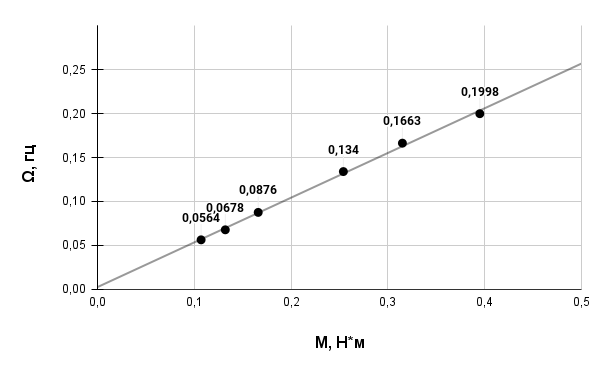
\includegraphics[scale=0.9]{Pics/picture3.png} \\
    \textit{\textcolor[HTML]{000000}{Рис. 3. График зависимости прецессии гироскопа от момента силы}}
\end{center}

Коэффициент $ k $ можно вычислить по следующей формуле:

\begin{equation}
k = \frac{\langle M\Omega\rangle}{\langle M^2 \rangle} \approx 0,518 \text{ } \frac{1}{\text{Дж} \cdot \text{с}}.
\end{equation}
Случайную погрешность определения $ k $ можно вычислить по следующей формуле:

\begin{equation}
\sigma^\text{сл}_k = \frac{1}{\sqrt{N_\text{оп}-1}} \sqrt{\frac{\langle \Omega^2 \rangle}{\langle M^2 \rangle} - k^2} \approx 0,0004 \text{ } \frac{1}{\text{Дж} \cdot \text{с}},
\end{equation}

Систематическую погрешность определения $ k $ можно вычислить следующим образом:

\begin{equation}
\sigma^\text{сист}_k = k\sqrt{\left( \frac{\sigma_M}{M} \right)^2+\left(\frac{\sigma_\Omega}{\Omega} \right)^2} \approx 0,0024 \text{ } \frac{1}{\text{Дж} \cdot \text{с}}.
\end{equation}

Тогда полная погрешность определения $ k $ определяется следующим образом:

\begin{equation}
\sigma_k = \sqrt{\left( \sigma_k^\text{сл} \right)^2 + \left( \sigma_k^\text{сист} \right)^2  } \approx 0,005 \text{ } \frac{1}{\text{Дж} \cdot \text{с}}.
\end{equation}

Таким образом, получаем:

\begin{itemize}
	\item \underline{$ k =\left( 0,518 \pm 0,005 \right) \frac{1}{\text{Дж} \cdot \text{с}} , \left( \varepsilon = 0,95 \% \right) $}
\end{itemize}

С помощью $ k $ можно вычислить угловую скорость вращения ротора гироскопа:

\begin{equation}
\omega_0 = \frac{1}{I_0 k} \approx 2475.0 \text{ с}^{-1},
\end{equation}
где $ I_0 $ -- момент инерции ротора гироскопа.

Тогда погрешность вычисления $ \omega_0 $ можно определить по формуле:

\begin{equation}
\sigma_{\omega_0} = \omega_0 \sqrt{\left( \frac{\sigma_{I_0}}{I_0} \right)^2 + \left( \frac{\sigma_k}{k} \right)^2} \approx 36.2 \text{ с}^{-1}.
\end{equation}

Таким образом, получаем:

\begin{itemize}
	\item \underline{$ \omega_0 =\left( 2475.0 \pm 36.2 \right) \text{ с}^{-1} , \left( \varepsilon = 1.46 \% \right) $}
\end{itemize}

Используя угловую скорость, можно определить частоту вращения ротора гироскопа:

\begin{equation}
\nu = \frac{\omega_0}{2\pi} \approx 393,9 \text{ Гц}.
\end{equation}

Погрешность определения частоты вращения вычисляется по следующей формуле:

\begin{equation}
\sigma_\nu = \nu \varepsilon_{\omega_0} \approx 5,5 \text{ Гц}.
\end{equation}

Таким образом, мы получили:

\begin{itemize}
	\item \underline{$ \nu = \left( 394 \pm 6 \right) \text{ Гц}, \left( \varepsilon = 1.52 \% \right)   $}
\end{itemize}

\section{Определение частоты вращения ротора гироскопа при помощи осциллографа}

Скорость вращения ротора гироскопа можно определить и не прибегая к исследованию прецессии. 
У используемых в работе гироскопов статор имеет две обмотки, необходимые для быстрой раскрутки гироскопа. 
В данном случае одну обмотку используют для раскрутки гироскопа, а вторую -- для измерения числа оборотов ротора. 
Ротор электромотора всегда немного намагничен. Вращаясь, он наводит во второй обмотке переменную ЭДС индукции, частота которой равна частоте вращения ротора. 
Частоту этой ЭДС измеряем по фигурам Лиссажу, получаемым на экране осциллографа, если на один вход подать исследуемую ЭДС, а на другой — переменное напряжение с хорошо прокалиброванного генератора. 
При совпадении частот на экране получится неподвижный эллипс.\\
При настройке генератора сигнала на частоту \underline{$ \nu_0 = 387.995$ Гц} на экране осциллографа виден  неподвижный эллипс, следовательно эта частота сигнала совпадает с частотой вращения ротора гироскопа.

\vspace*{0.3cm}

{\large Момент силы трения}

Исследуем зависимость опускания оси гироскопа от времени.

\begin{table}[h!]
	\centering
	\begin{tabular}{|c|c|c|c|c|c|c|c|c|}
		\hline
	№  & $\alpha$, рад & $\sigma_{\alpha}$, рад & $t$, с & $\sigma$, c & $\overline{T}, c$ & $\sigma_T$, c & $\varOmega$ рад/с & $\sigma_{\varOmega}$, рад/с	\\ \hline
	1  & 0.209 & 0.017 & 264.09 & 0.3 & 263.87 & 0.43 & 0.792 & 0.06 \\ \hline
	2  & 0.209 & 0.017 & 263.65 & 0.3 & 263.87 & 0.43 & 0.792 & 0.06 \\ \hline
	\end{tabular}
	\caption{Результат измерения зависимости опускания оси гироскопа от времени}
\end{table}

Момент силы силы трения можно посчитать по формуле 

\begin{equation}
	M = \varOmega I_0\omega_0 = \frac{\varOmega}{k} \approx 1.5 \cdot 10^{-3} H*\text{м}
\end{equation}

Его погрешность считается по формуле

\begin{equation}
	\sigma_M = M \sqrt{(\frac{\sigma_k}{k})^2 + (\frac{\sigma_{\varOmega}}{\varOmega})^2} \approx 1.5 \cdot 10^{-5} \text{}
\end{equation}

Полученное значение момента силы трения, очевидно, мало относительно значения момента силы тяжести.
Однако, сила трения действует в сторону направления действия силы тяжести, поэтому для получения более точных результатов пренебрегать ею не стоит.

\section{Вывод}
В ходе работы мы получили частоту вращения ротора гироскопа. К сожалению, в случае с измерением частоты с помощью осциллографа, ее точное значение измерить не удалось.
Однако, мы смогли получить нижнюю границу значения частоты. Как и было ожидаемо изначально,
частота вращения, полученная первым способом, оказалась больше частоты, полученной с помощью осциллографа.

\end{document}